\section{Case study}

To show the functionality and applicability of the automatic domain decomposition library a few case studies were carried out.
This chapter and the following sections will outline each case study and the corresponding experimental results.

The base implementation of each test case was provided by Stefano Ubbiali written in Python and using GT4Py stencils.

\subsection{Case 1: Burger's equation}
Burger's equation is a well-known nonlinear partial differential equation.
Burger's equation can be used to model various physical phenomena.
Most commonly it is used as a model for traffic flow or shock waves in a fluid.
Additionally it is widely used to test numerical schemes since it has analytical solutions for a set of initial conditions.

\subsubsection{Case description}
\label{sec:case_description}

The two-dimensional, viscid Burger's equation is given by the following system of scalar equations as described in \citet{zhao2011new}:

\begin{equation}
\begin{split}
\pdv{u}{t} + u \pdv{u}{x} + v \pdv{u}{y} = \varepsilon \left( \pdv{^2 u}{x^2} + \pdv{^2 u}{y^2} \right) \\
\pdv{v}{t} + u \pdv{v}{x} + v \pdv{v}{y} = \varepsilon \left( \pdv{^2 v}{x^2} + \pdv{^2 v}{y^2} \right) \\
\text{with } \left(x, y, t\right) \in D \times \left(0,T\right]
\end{split}
\end{equation}

These two equations characterize the Burger equation as a set of equations for the velocity in x and y direction.
Both equations consist of two parts.
On the left hand side, the advection of the velocity itself.
On the right hand side, the diffusion caused by viscosity.

To complete the full description of the Burger equation the initial and boundary conditions are generally given in the following form:

\begin{equation}
\begin{split}
\text{Initial conditions: } \\
u\left(x, y, 0\right) = u_0\left(x, y\right) \text{, } \left(x, y\right) \in D \\
v\left(x, y, 0\right) = v_0\left(x, y\right) \text{, } \left(x, y\right) \in D \\
\text{Boundary conditions: } \\
u\left(x, y, t\right) = f\left(x, y, t\right) \text{, } \left(x, y, t\right) \in \partial D \times \left(0, T\right] \\
v\left(x, y, t\right) = g\left(x, y, t\right) \text{, } \left(x, y, t\right) \in \partial D \times \left(0, T\right]
\end{split}
\end{equation}

\paragraph{Shankar conditions:}

The first set of initial and boundary conditions are the ones used by Shankar. 
\footnote{https://ch.mathworks.com/matlabcentral/fileexchange/38087-burgers-equation-in-1d-and-2d Accessed: 25.9.18}

The following equations describe the Shankar test case fully and Fig. \ref{fig:shankar_ic1} and Fig. \ref{fig:shankar_ic2} visualizes the initial condition.

\begin{equation}
\begin{tabular}{l l}
\text{\textbf{Boundary conditions: }} 
& 
\text{\textbf{Initial conditions: }} 
\\
f\left(x, y, t\right) = 0 
&
u_0\left(x, y\right) = \begin{cases}
0, \text{ in } \left[0.5, 1.0\right] \times \left[0.5, 1.0\right] \\
1, \text{ otherwise}
\end{cases}
\\
g\left(x, y, t\right) = 0 
&
v_0\left(x, y\right) =  \begin{cases}
1, \text{ in } \left[0.5, 1.0\right] \times \left[0.5, 1.0\right] \\
0, \text{ otherwise}
\end{cases}
\\
\text{\textbf{Other parameters: }} 
&
\text{\textbf{Domain: }}
\\
\text{Viscosity: } \varepsilon = 0.01
&
D = \left[0,2\right] \times \left[0,2\right] 
\\
&
T = 0.6
\end{tabular}
\end{equation}

\begin{figure}
\centering
\begin{subfigure}{.5\textwidth}
  \centering
  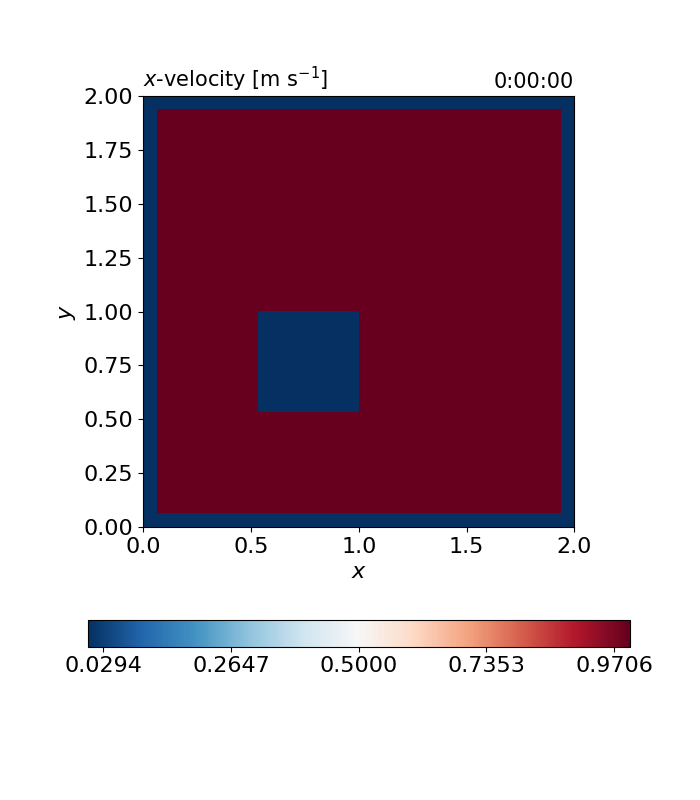
\includegraphics[width=1.1\linewidth]{test_shankar_forward_backward_field_u_at_0.png}
  \caption{X-velocity initial condition.}
  \label{fig:shankar_ic1}
\end{subfigure}%
\begin{subfigure}{.5\textwidth}
  \centering
  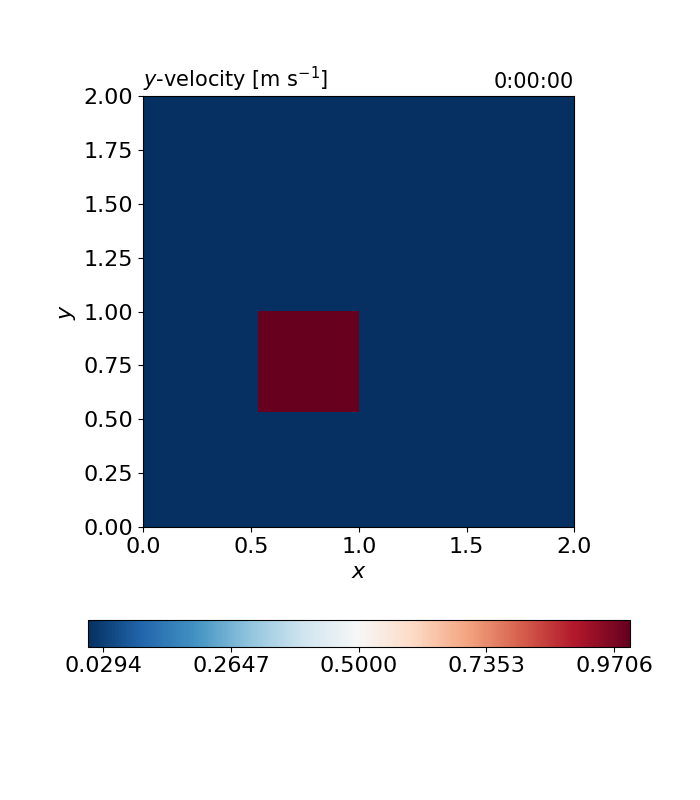
\includegraphics[width=1.1\linewidth]{test_shankar_forward_backward_field_v_at_0.png}
  \caption{Y-Velocity initial condition.}
  \label{fig:shankar_ic2}
\end{subfigure}
\caption{Initial condition for the Shankar test case.}
\label{fig:shankar_ic}
\end{figure}

\newpage
\paragraph{Zhao conditions:}

The second set of initial and boundary conditions are the same as used as example 1 in \citet{zhao2011new}:

\begin{equation}
\begin{tabular}{l l}
\text{\textbf{Boundary conditions: }} & \text{\textbf{Initial conditions: }} \\
f\left(x, y, t\right) = \begin{cases}
-2 \varepsilon \pi \exp^{-5 \pi^2 \varepsilon t} \sin\left(\pi y\right) \text{, for } x = 0, y \in \left[0, 1\right] \\
-2 \varepsilon \pi \exp^{-5 \pi^2 \varepsilon t} \sin\left(\pi y\right) \text{, for } x = 1, y \in \left[0, 1\right] \\
0 \text{, for } x \in \left[0, 1\right], y = 0 \\
0 \text{, for } x \in \left[0, 1\right], y = 1 \\
\end{cases}
& 
u_0\left(x, y\right) = \frac{-4 \varepsilon \pi \cos \left(2 \pi x\right) \sin \left(\pi y\right)}{2 + \sin \left(2 \pi x \right) \sin \left(\pi y\right)}
\\
g\left(x, y, t\right) = \begin{cases}
0 \text{, for } x = 0, y \in \left[0, 1\right] \\
0 \text{, for } x = 1, y \in \left[0, 1\right] \\
-\varepsilon \pi \exp^{-5 \pi^2 \varepsilon t} \sin\left(2 \pi x\right) \text{, for } x \in \left[0, 1\right], y = 0 \\
\varepsilon \pi \exp^{-5 \pi^2 \varepsilon t} \sin\left(2 \pi x\right) \text{, for } x \in \left[0, 1\right], y = 1 \\
\end{cases}
&
v_0\left(x, y\right) = \frac{-2 \varepsilon \pi \sin \left(2 \pi x\right) \cos \left(\pi y\right)}{2 + \sin \left(2 \pi x \right) \sin \left(\pi y\right)}
\\
\text{\textbf{Other parameters: }} & \text{\textbf{Domain: }}
\\
\text{Viscosity: } \varepsilon = 0.01
& D = \left[0,1\right] \times \left[0,1\right]
\\
 & T = 1
\end{tabular}
\end{equation}

\begin{figure}
\centering
\begin{subfigure}{.5\textwidth}
  \centering
  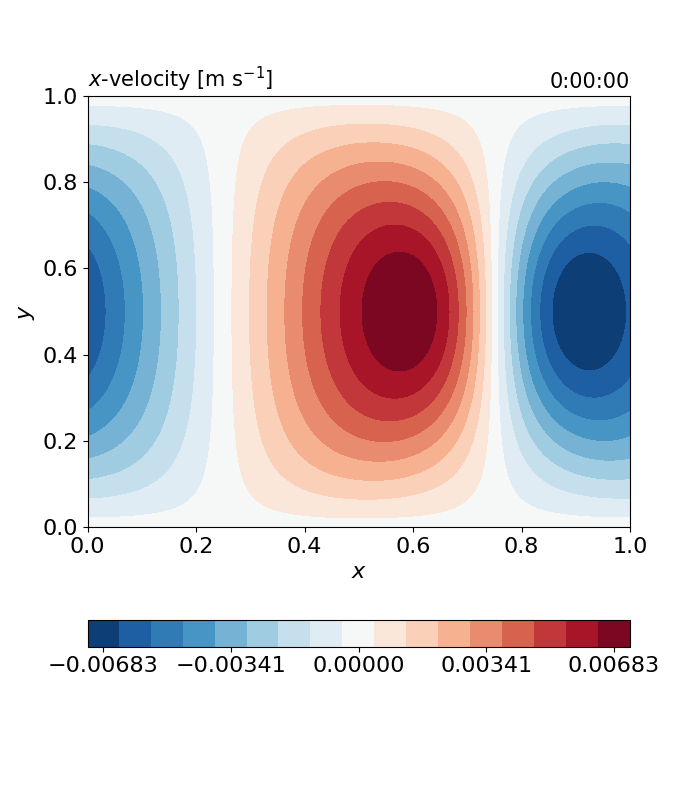
\includegraphics[width=1.1\linewidth]{test_zhao_forward_backward_field_u_at_0.png}
  \caption{X-velocity initial condition.}
  \label{fig:zhao_ic1}
\end{subfigure}%
\begin{subfigure}{.5\textwidth}
  \centering
  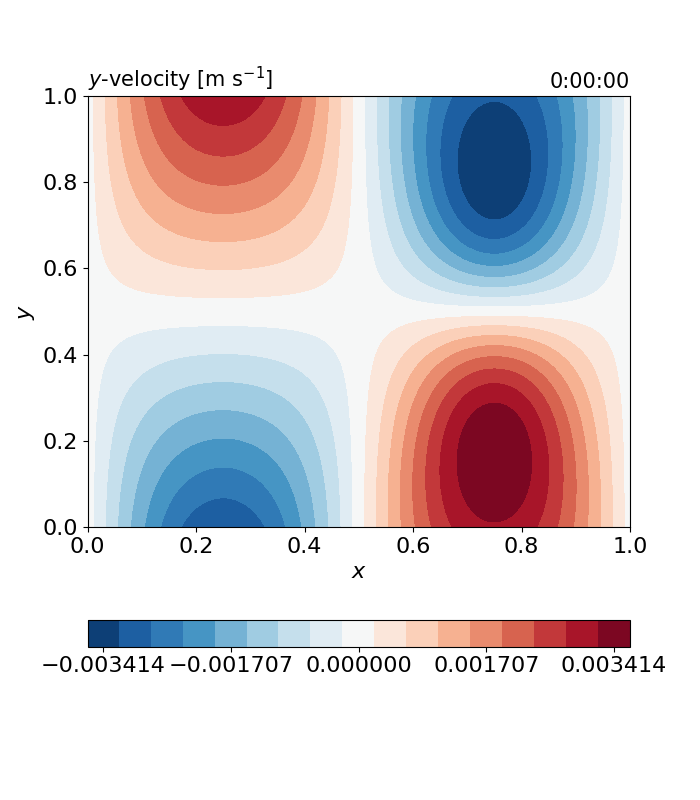
\includegraphics[width=1.1\linewidth]{test_zhao_forward_backward_field_v_at_0.png}
  \caption{Y-Velocity initial condition.}
  \label{fig:zhao_ic2}
\end{subfigure}
\caption{Initial condition for the Zhao test case.}
\label{fig:zhao_ic}
\end{figure}

Notable about this set of initial and boundary condition is that they admit exact solutions.
The exact solutions as provided in \citet{zhao2011new} are:
\\
\begin{equation}
\label{eq:exact_solution}
\begin{split}
u\left(x,y,t\right) = -2\varepsilon \frac{2 \pi \exp^{-5 \pi^2 \varepsilon t} \cos\left(2 \pi x\right) \sin\left(\pi y\right)}{2 + \exp^{-5 \pi^2 \varepsilon t}\sin\left(2 \pi x\right) \sin\left(\pi y\right)}
\\
v\left(x,y,t\right) = -2\varepsilon \frac{\pi \exp^{-5 \pi^2 \varepsilon t} \sin\left(2 \pi x\right) \cos\left(\pi y\right)}{2 + \exp^{-5 \pi^2 \varepsilon t}\sin\left(2 \pi x\right) \sin\left(\pi y\right)}
\end{split}
\end{equation}

\subsubsection{Implementation details}
\paragraph{Stencil details: }
Both the Shankar and Zhao conditions can be solved using different numerical stencils for the computation.
To show some variance and flexibility three stencils can be used to solve the test case.

The forward-backward stencil combines forward finite differences to compute the time derivatives with backward finite differences to compute the first-order space derivatives and a second-order centered scheme to compute the second-order derivatives.
See Fig. \ref{fig:fb_stencil} for a visual representation of this stencil.

The other two stencil are called upwind schemes, since they use the values only from the direction the velocity is coming from.
The first-order upwind scheme uses the directly neighboring grid points like the forward-backward stencil.
The difference is that only the values from upwind are used in the actual computation for the next value.
See Fig. \ref{fig:upwind_stencil} for a visual representation of this stencil.

The third-order upwind stencil needs two neighboring grid points in each direction to increase the accuracy of the approximated space derivative.
See Fig. \ref{fig:upwind_third_stencil} for a visual representation of this stencil.

\begin{figure}[!htbp]
\centering
\begin{subfigure}{.3\textwidth}
  \centering
  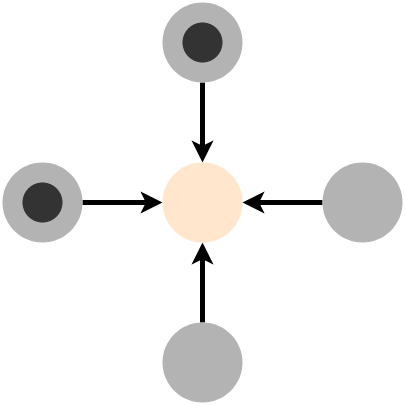
\includegraphics[width=0.8\linewidth]{fb_stencil.png}
  \caption{Forward-backward}
  \label{fig:fb_stencil}
\end{subfigure}%
\begin{subfigure}{.3\textwidth}
  \centering
  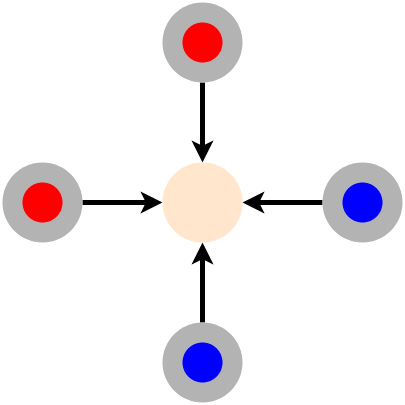
\includegraphics[width=0.8\linewidth]{upwind.png}
  \caption{Upwind first order}
  \label{fig:upwind_stencil}
\end{subfigure}
\begin{subfigure}{.3\textwidth}
  \centering
  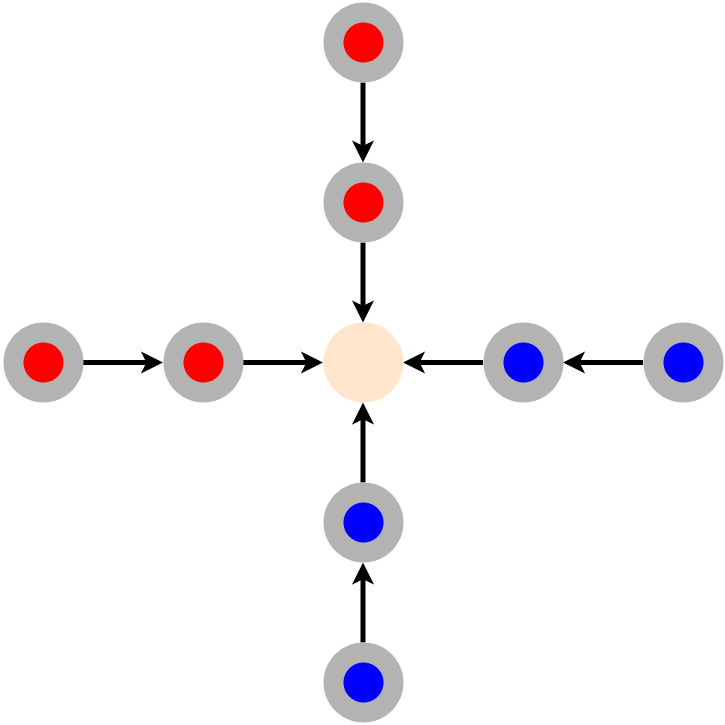
\includegraphics[width=0.8\linewidth]{upwind_third.png}
  \caption{Upwind third order}
  \label{fig:upwind_third_stencil}
\end{subfigure}
\caption{Schematic representation for three possible stencils for the Burger's equation. The large gray circle indicate the grid points necessary for the computation of the Laplacian for the diffusion part of the Burger's equation. The small dark gray circle indicate grid points necessary for the backward finite difference. The red and blue small circles indicate grid points needed for the upwind computations in the case of positive velocity or negative velocity respectively.}
\label{fig:burger_stencils}
\end{figure}

\subsubsection{Validation}
Changing stencil computation from serial to distributed can cause various errors to appear.
Therefore, it is important to validate the solutions obtained using the domain decomposition library against reference solutions.

\paragraph{Comparison with the exact solution} is a useful tool to validate any stencil code.
The Burger's equation and specifically the Zhao setup presented before provide such reference and exact solutions.

Figure \ref{fig:burgers_validation} shows these validation results. The first four plots in Fig. \ref{fig:burgers_validation} show the spatial distribution of the error of either the domain decomposed solution (left panel) or the reference solution (right panel).
This is an actual error since it compares the computed solutions against the analytical, exact solution.

This comparison is done to verify that the addition of internal boundaries between subdivisions does not add to the spatial error distribution of the computation.
These particular plots were generated using 16 subdivisions but the same plots for 8, 4, or 32 subdivisions show the same results.

Additionally, Fig. \ref{fig:burgers_val5} and Fig. \ref{fig:burgers_val6} show the spatial distribution of the difference between the reference solution and the domain decomposed solution.
There is a difference between the reference solution and the domain decomposed solution because decomposing the domain necessarily changes the ordering of some computations causing the difference due to floating point operations not guaranteeing bit identical results.
The spatial distribution of this difference is not identical between the velocity u (shown in Fig. \ref{fig:burgers_val5}) and velocity v (shown in Fig. \ref{fig:burgers_val6})

Not shown here is a plot comparing different setups of the domain decomposed solution e.g. the difference between all subdivisions belonging to the same partition (i.e. only local communication) and subdivisions belonging to multiple partitions (i.e. MPI communication).
These plots are not shown because they would show no spatial distribution and instead a difference of zero everywhere.
Meaning that for the same number of subdivisions the way of communicating their boundaries between each other has no influence on the computation and produces bit-identical results as expected.

\begin{figure}[!htbp]
\centering
\begin{subfigure}{0.45\textwidth}
  \centering
  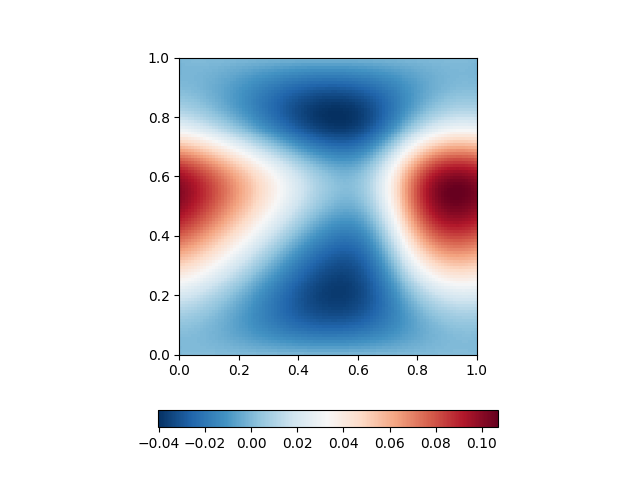
\includegraphics[width=\linewidth]{zhao_exact_vs_dd_time_avg_field_u.png}
  \caption{Difference in velocity u field between exact solution and domain decomposed solution averaged over all time steps.}
  \label{fig:burgers_val1}
\end{subfigure} \hfill
\begin{subfigure}{0.45\textwidth}
  \centering
  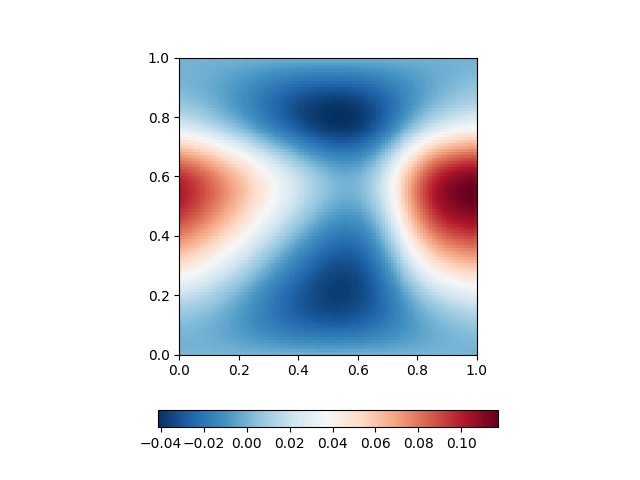
\includegraphics[width=\linewidth]{zhao_exact_vs_ref_time_avg_field_u.png}
  \caption{Difference in velocity u field between exact solution and reference solution averaged over all time steps.}
  \label{fig:burgers_val2}
\end{subfigure}

\begin{subfigure}{0.45\textwidth}
  \centering
  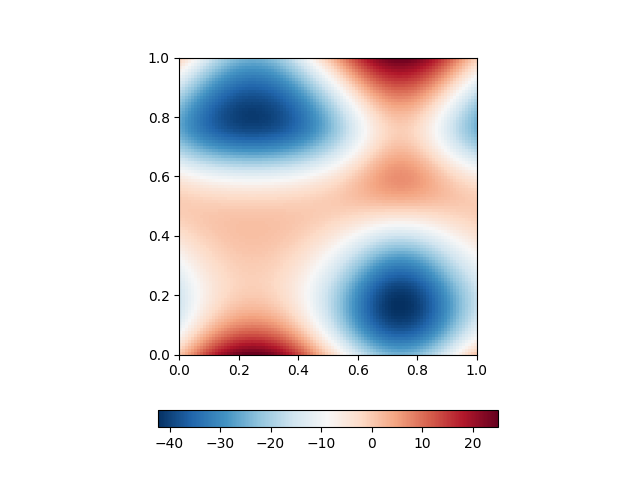
\includegraphics[width=\linewidth]{zhao_exact_vs_dd_time_avg_field_v.png}
  \caption{Difference in velocity v field between exact solution and domain decomposed solution averaged over all time steps.}
  \label{fig:burgers_val3}
\end{subfigure} \hfill
\begin{subfigure}{0.45\textwidth}
  \centering
  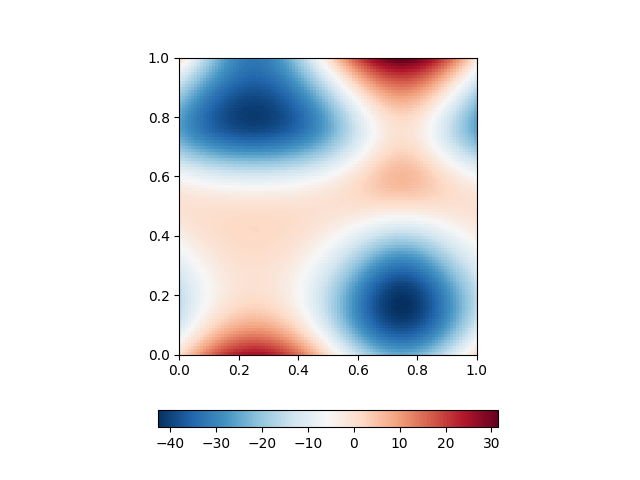
\includegraphics[width=\linewidth]{zhao_exact_vs_ref_time_avg_field_v.png}
  \caption{Difference in velocity v field between exact solution and reference solution averaged over all time steps.}
  \label{fig:burgers_val4}
\end{subfigure}

\begin{subfigure}{0.45\textwidth}
  \centering
  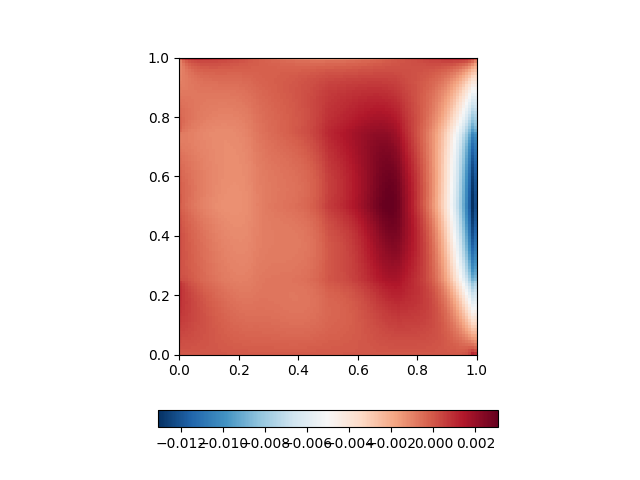
\includegraphics[width=\linewidth]{zhao_ref_vs_dd_time_avg_field_u.png}
  \caption{Difference in velocity u field between reference solution and domain decomposed solution averaged over all time steps.}
  \label{fig:burgers_val5}
\end{subfigure} \hfill
\begin{subfigure}{0.45\textwidth}
  \centering
  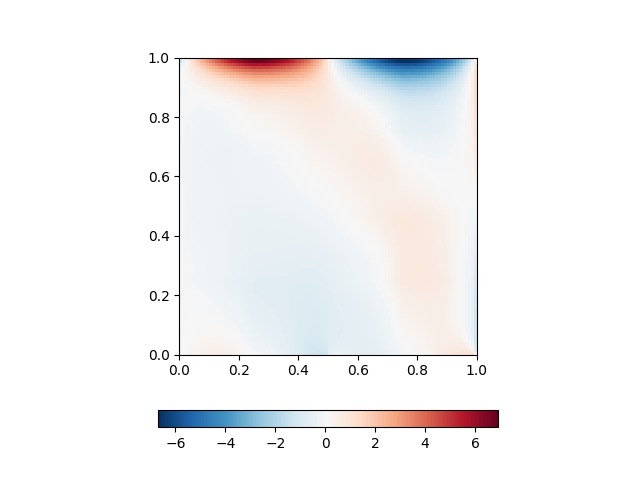
\includegraphics[width=\linewidth]{zhao_ref_vs_dd_time_avg_field_v.png}
  \caption{Difference in velocity v field between reference solution and domain decomposed solution averaged over all time steps.}
  \label{fig:burgers_val6}
\end{subfigure}
\caption{Burger's equation Zhao Setup. 
Exact solution refers to the analytical solution shown in Eq. \ref{eq:exact_solution}.
Reference refers to solutions computed using the original, serial Python and GridTools4Py version.
Lastly, domain decomposed solution refers to solutions computed using the domain decomposition library.
The domain size for this validation is 100 by 100 grid points and the computations are run for 1000 time steps.
}
\label{fig:burgers_validation}
\end{figure}


\begin{figure}[!htbp]
\centering
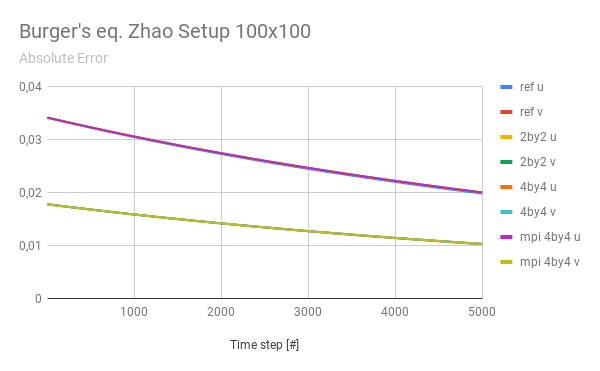
\includegraphics[width=\linewidth]{Absolute_Error_Time_Evolution.png}
\caption{Time evolution of the absolute error in a Burger's equation Zhao setup for the reference code and a few different versions of the domain decomposed code.}
\label{fig:burgers_time_evolution}
\end{figure}

\paragraph{Error time evolution:}
The previous plots have focused on the spatial distribution of differences because any coding errors in the subdivision boundary exchange would clearly show up in these comparisons.
However, changing the code from serial to domain decomposed could potentially introduce erroneous numerical diffusion.
Such an error would increase over many time steps.
Therefore, Fig. \ref{fig:burgers_time_evolution} shows that the error does not increase in later time steps.
The absolute error shown here in fact decreases over time since the solution as a whole decreases over time due to physical diffusion in the Burger's equation.

The time evolution of the error in Fig. \ref{fig:burgers_time_evolution} was measured for the reference solution, a 4 subdivision and 16 subdivision solutions with only local communication, as well as a 16 subdivision solution with MPI communication.
However, the behavior of the absolute error over time is so similar between all of these that in the lines in Fig. \ref{fig:burgers_time_evolution} overlap for all u velocity solutions and all v velocity solutions.

The difference to the exact solution has a spatial distribution because it originates in the discretization of the analytical initial condition and computations.
This relationship between the error and the grid discretization can be used to validate the domain decomposed solutions by performing a grid refinement study.

\paragraph{Grid refinement study} is a method to validate code most commonly used in computational fluid mechanics.
In a grid refinement study the error of a computation is calculated on various grid sizes that are made smaller by a factor.
It is most common to half the grid spacing per measurement.
If this refinement is done in the asymptotic range of convergence for a stencil then the leading term of the truncation error dominates the overall error.
This means that if error for each grid spacing is plotted in a log-log plot the slope of the line is the measured order of accuracy and if the implementation is correct should be equal to the theoretical order of accuracy of the stencil.

Figure \ref{fig:grs} shows such a grid refinement study for the Burger's equation Zhao setup.
Note that both the forward-backward and the upwind stencil have an order of accuracy of 2.
The upwind third-order stencil should have, as the name suggests, an order of accuracy of 3.
However, this is only the order of accuracy of the spatial stencil.
Since the Burger's equation Zhao setup uses a very simple first-order in time discretization the measured order of accuracy for the third-order upwind scheme is limited by the time discretization.

\begin{figure}[!htbp]
\centering
\begin{subfigure}{0.8\textwidth}
  \centering
  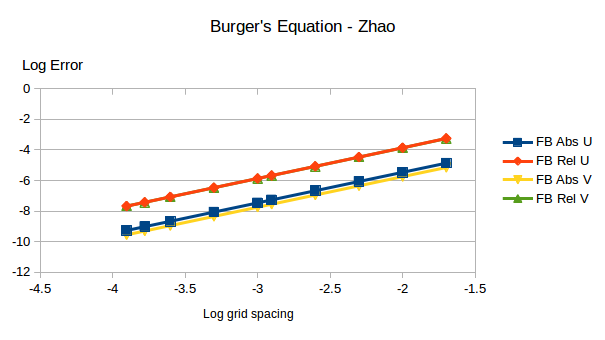
\includegraphics[width=\linewidth]{GRS_FB.png}
  \caption{Grid refinement for the forward-backward stencil.}
  \label{fig:grs_1}
\end{subfigure}

\begin{subfigure}{0.8\textwidth}
  \centering
  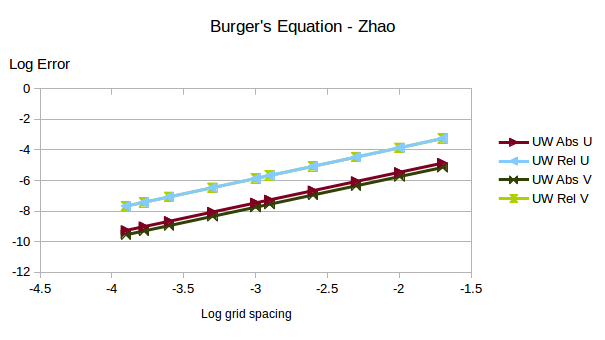
\includegraphics[width=\linewidth]{GRS_UW.png}
  \caption{Grid refinement for the upwind stencil.}
  \label{fig:grs_2}
\end{subfigure}

\begin{subfigure}{0.8\textwidth}
  \centering
  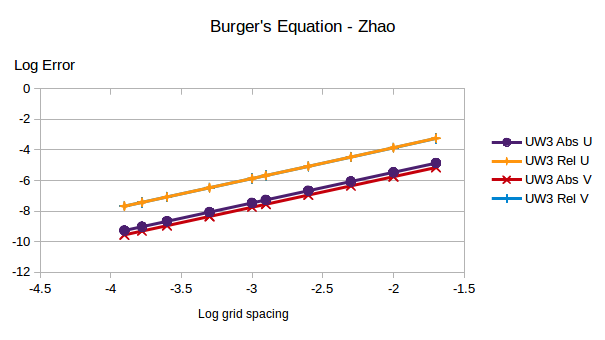
\includegraphics[width=\linewidth]{GRS_UW3.png}
  \caption{Grid refinement for the upwind third-order stencil.}
  \label{fig:grs_3}
\end{subfigure}
\caption{Grid refinement study of the Burger's equation Zhao setup for the three stencils described before.}
\label{fig:grs}
\end{figure}

\subsubsection{Performance and Scalability}

\paragraph{Weak scaling}

\begin{table}[!htbp]
\centering
\ra{1.5}
\begin{tabular}{l r r r r r r r}
\toprule
Name & GP per Dim [$10^3$] & Total GP [$10^7$] & Nodes & Tasks & SD x & SD y \\
\midrule
1N1T	&	4	&	1.6	&	1	&	1	&	0	&	0	\\
1N2T	&	5.66	&	3.2	&	1	&	2	&	2	&	1	\\
1N4T	&	8	&	6.4	&	1	&	4	&	2	&	2	\\
1N6T	&	9.8	&	9.6	&	1	&	6	&	3	&	2	\\
1N8T	&	11.3	&	12.8	&	1	&	8	&	4	&	2	\\
2N12T	&	13.9	&	19.2	&	2	&	12	&	4	&	3	\\
2N16T	&	16	&	25.6	&	2	&	16	&	4	&	4	\\
3N18T	&	17	&	28.8	&	3	&	18	&	6	&	3	\\
3N24T	&	19.6	&	38.4	&	3	&	24	&	6	&	4	\\
4N24T	&	19.6	&	38.4	&	4	&	24	&	6	&	4	\\
4N32T	&	22.7	&	51.2	&	4	&	32	&	8	&	4	\\
5N30T	&	21.9	&	48	&	5	&	30	&	6	&	5	\\
5N40T	&	25.3	&	64	&	5	&	40	&	8	&	5	\\
6N36T	&	24	&	57.6	&	6	&	36	&	6	&	6	\\
6N48T	&	27.7	&	76.8	&	6	&	48	&	8	&	6	\\
7N42T	&	26	&	67.2	&	7	&	42	&	7	&	6	\\
7N56T	&	30	&	89.6	&	7	&	56	&	8	&	7	\\
8N48T	&	27.7	&	76.8	&	8	&	48	&	8	&	6	\\
8N64T	&	32	&	102	&	8	&	64	&	8	&	8	\\
\bottomrule
\end{tabular}
\caption{Setup for the first weak scaling experiment run on Greina.}
\label{tab:weak_4k}
\end{table}

\begin{table}[!htbp]
\centering
\ra{1.5}
\begin{tabular}{l r r r r r r r}
\toprule
Name & GP per Dim [$10^3$] & Total GP [$10^7$] & Nodes & Tasks & SD x & SD y \\
\midrule
1N1T	&	5	&	2.5	&	1	&	1	&	0	&	0	\\
1N2T	&	7	&	5	&	1	&	2	&	2	&	1	\\
1N4T	&	10	&	10	&	1	&	4	&	2	&	2	\\
1N6T	&	12	&	15	&	1	&	6	&	3	&	2	\\
1N8T	&	14	&	20	&	1	&	8	&	4	&	2	\\
2N12T	&	16.8	&	30	&	2	&	12	&	4	&	3	\\
2N16T	&	20	&	40	&	2	&	16	&	4	&	4	\\
3N18T	&	20.9	&	45	&	3	&	18	&	6	&	3	\\
3N24T	&	24	&	60	&	3	&	24	&	6	&	4	\\
4N24T	&	24	&	60	&	4	&	24	&	6	&	4	\\
4N32T	&	28	&	80	&	4	&	32	&	8	&	4	\\
5N30T	&	27	&	75	&	5	&	30	&	6	&	5	\\
5N40T	&	32	&	100	&	5	&	40	&	8	&	5	\\
6N36T	&	31	&	90	&	6	&	36	&	6	&	6	\\
6N48T	&	34.6	&	120	&	6	&	48	&	8	&	6	\\
%7N42T	&	26	&	67.2	&	7	&	42	&	7	&	6	\\
7N56T	&	37.3	&	140	&	7	&	56	&	8	&	7	\\
8N48T	&	34.6	&	120	&	8	&	48	&	8	&	6	\\
8N64T	&	40	&	160	&	8	&	64	&	8	&	8	\\
\bottomrule
\end{tabular}
\caption{Setup for the second weak scaling experiment run on Greina.}
\label{tab:weak_5k}
\end{table}

